% Součást skript Datové struktury. ds.tex
% Authors: Martin Vidner
%	   Vladimir Kotal
\markright{$ $Id$ $}

\chapter{$(a,b)$ stromy}

% --------------------------------------------------------------------------
\section{Základní varianta}

Nechť $a, b \in \mathbb{N}, a \leq b$. Strom je $(a,b)$ strom, když
platí
\begin{enumerate}
\item Každý vnitřní vrchol kromě kořene má alespoň $a$ a nejvýše $b$
synů.
\item Kořen má nejvýše $b$ synů. Pokud $a \geq 2$, pak má alespoň 2
syny, nebo je listem.
\item Všechny cesty z kořene do listu jsou stejně dlouhé.
\end{enumerate}
\exercise
{Co by se stalo, kdybychom definici zjednodušili a místo podmínek 1 a
2 požadovali, aby \emph{každý} vrchol měl $a$ až $b$ synů?}{Nebyly by
možné malé $(a,b)$ stromy.}

\begin{figure}%[!htb]
\centering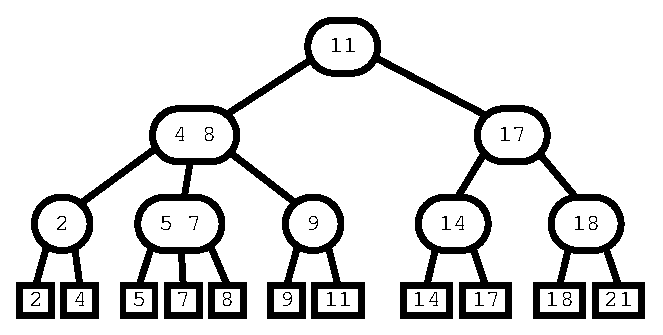
\includegraphics{pics/abt}
\caption{Příklad $(a,b)$ stromu}
\label{abt}
\end{figure}

\begin{defn}
Jsou-li synové každého vrcholu očíslováni, můžeme
definovat \emph{lexikografické uspořádání vrcholů na stejné hladině}.

$u \leq_l v$, jestliže $\text{otec } u <_l \text{otec } v$ nebo
$\text{otec } u = \text{otec } v$, $u$ je $i$-tý syn, $v$ je $j$-tý syn
a $i \leq j$.
\end{defn}

\begin{pozn}
Prvky z množiny $S$ korespondují s listy $T$ tak, že $s < s', s,s' \in S$,
právě když list odpovídající $s <_l$ list odpovídající $s'$.
\end{pozn}

Pozorování: Buď $T$ $(a,b)$ strom s hloubkou $h$. Platí
\[
2 a^{h-1} \leq \text{počet listů $T$} \leq  b^h,
\]
tedy pro libovolné $n$ má každý $(a,b)$ strom $T$ s $n$ listy 
hloubku $\Theta(\log n)$.

% ..........................................................................
\subsection{Reprezentace množiny $S$ $(a,b)$ stromem}

Mějme $S \subseteq U$, přičemž universum je lineárně uspořádané.
$(a,b)$ strom $T$ reprezentuje množinu $S$, jestliže existuje
jednoznačné přiřazení prvků $S$ listům $T$, které zachovává uspořádání.

Potřebujeme navíc podmínku
\begin{enumerate}
\item[4.] $a \geq 2$ a $b \geq 2a - 1$ 
\end{enumerate}

Struktura vnitřního vrcholu $v$:
\begin{itemize}
\item $\rho_v$ je počet synů
\item $S_v[1\ .. \ \rho_v]$ je pole ukazatelů na syny
\item $H_v[1\ .. \ \rho_v - 1]$: $H_v[i]$ je maximální prvek 
v~podstromu $S_v[i]$ 
\end{itemize}

% ..........................................................................
\subsection{MEMBER($x$) v $(a,b)$ stromu}

viz algoritmus \ref{alg:abtree.member}

\begin{algorithm}[!htb]
\caption{MEMBER pro $(a,b)$ stromy}
\label{alg:abtree.member}
\begin{algorithmic}
\STATE \COMMENT{vyhledání $x$}
\STATE $t := \text{kořen}$
\WHILE {$t$ není list}
	\STATE $i := 1$
	\WHILE {$H_t[i] < x \land i < \rho_t$}
		\STATE $i := i + 1$
	\ENDWHILE
	\STATE $t := S_t[i]$ 
\ENDWHILE
\STATE \COMMENT{testování $x$}
\IF {$t$ reprezentuje $x$}
	\STATE $x \in S$
\ELSE
	\STATE $x \notin S$
\ENDIF
\end{algorithmic}
\end{algorithm}

% ..........................................................................
\subsection{INSERT($x$) do $(a,b)$ stromu}

viz algoritmus \ref{alg:abtree.insert}

\begin{algorithm}[!htb]
\caption{INSERT pro $(a,b)$ stromy}
\label{alg:abtree.insert}
\begin{algorithmic}
\STATE vyhledání $x$
\IF {$t$ nereprezentuje $x$}
	\STATE $o := \text{otec } t$
	\STATE vrcholu $o$ přidej nového syna $t'$ 
	reprezentujícího $x$
	\STATE zařaď $t'$ na správné místo mezi jeho bratry
	a uprav $\rho_o$, $S_o$ a $H_o$
	\STATE $t := o$
	\WHILE {$\rho_t > b$}
		\STATE \COMMENT {Štěpení 
				--- můžeme provést díky podmínce 4}
		\STATE rozděl $t$ na $t_1$ a $t_2$ 
		\STATE \quad k $t_1$ dej prvních 
			$\lfloor (b+1)/2 \rfloor$ synů $t$
		\STATE \quad k $t_2$ dej zbylých 
			$\lceil (b+1)/2 \rceil$ synů $t$
		\STATE $o := \text{otec } t$
		\STATE uprav $\rho_o$, $S_o$ a $H_o$
		\STATE \COMMENT {při štěpení kořene ještě musíme
				vytvořit nový kořen}
		\STATE $t := o$
	\ENDWHILE
\ENDIF
\end{algorithmic}
\end{algorithm}

% ..........................................................................
\subsection{DELETE($x$) z $(a,b)$ stromu}

viz algoritmus \ref{alg:abtree.delete}

\begin{algorithm}[!htb]
\caption{DELETE pro $(a,b)$ stromy}
\label{alg:abtree.delete}
\begin{algorithmic}
\STATE vyhledání $x$, navíc si zapamatuj vrchol $u$, 
	v jehož poli $H_u$ je $x$
\IF {$t$ reprezentuje $x$}
	\STATE $o := \text{otec } t$
	\STATE odstraň $t$
	\STATE uprav $H_o$, $H_u$ \COMMENT {...}
	\STATE uprav $S_o$ a $\rho_o$
	\STATE $t := o$
	\WHILE {$\rho_t < a \land t \text{ není kořen}$}
		\STATE $v := \text{bezprostřední bratr } t$ 
		\IF[smíme spojit] {$\rho_v = a$}
			\STATE \COMMENT {Spojení}
			\STATE $o := \text{otec } t$
			\STATE sluč $v$ a $t$ do $t$
			\STATE uprav $\rho_o$, $S_o$ a $H_o$
			\STATE $t := o$
		\ELSE[$\rho_v > a$, spojení by mohlo mít více než $b$ synů]
			\STATE \COMMENT {Přesun}
			\STATE přesuň krajního syna $v$ do $t$
			\STATE uprav $H_{\text{otec } t}$
		\ENDIF
	\ENDWHILE
	\IF {$t$ je kořen a má jen jednoho syna}
		\STATE smaž $t$
	\ENDIF
\ENDIF
\end{algorithmic}
\end{algorithm}

% ..........................................................................
\subsection{Shrnutí}

Operace štěpení, přesun i spojení vyžadují konstantní čas. 
\begin{theorem}
Operace MEMBER, INSERT a DELETE pro $(a,b)$ stromy vyžadují čas
$O(\log n)$, kde $n$ je velikost reprezentované množiny.
\end{theorem}

S $H$ a $S$ jsme pracovali jako se seznamy, nepotřebujeme, aby to byla
pole. Tím se zjednoduší implementace. 
\mnote{Výhodnost pro vnější paměti?}

% ..........................................................................
\subsection{Jak volit parametry $(a,b)$}

Pro vnitřní paměť je vhodné $a = 2$ nebo $a=3$, $b = 2a$.
Pro vnější paměť je vhodné $a \approx 100$, $b = 2a$.

Pro minimalizaci paměťových nároků je výhodné $b = 2a-1$,
pro minimalizaci časových nároků je výhodné $b = 2a$.
\mnote{proč? prý se k tomu ještě dostaneme}

% --------------------------------------------------------------------------
\section{Další operace}

MIN, MAX (XXX)

% ..........................................................................
Pro operaci JOIN je vhodné spolu se stromem uchovávat také 
největší prvek reprezentované množiny.

\subsection{Algoritmus JOIN($T_1, T_2$) pro $(a,b)$ stromy}

Operace JOIN provede spojení dvou (a,b)-stromů $T_1$ a $T_2$ 
do jednoho (a,b)-stromu za předpokladu, že všechny prvky, které 
reprezentuje strom $T_1$ jsou menší než prvky reprezentované stromem
$T_2$.

Algoritmus najde vrchol pro stromu $T_2$, spojí stromy do jednoho (viz
obr. \ref{fig:abtree.join}) a provede štěpění.

\begin{figure}
\centering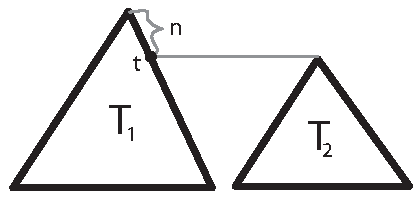
\includegraphics{pics/abtree-join}
\caption{Idea operace JOIN}
\label{fig:abtree.join}
\end{figure}

Přepis viz algoritmus \ref{alg:abtree.join}

\begin{algorithm}[!htb]
\caption{JOIN pro $(a,b)$ stromy}
\label{alg:abtree.join}
\begin{algorithmic}
\REQUIRE {$T_1$ reprezentuje $S_1$, $T_2$ reprezentuje $S_2$ 
	a $\max S_1 < \min S_2$ }
\STATE $n := \text{hloubka } T_1 - \text{hloubka } T_2$ 
\IF {$n \geq 0$}
	\STATE $t := \text{kořen } T_1$
	\WHILE {$n > 0$}
		\STATE $t := \text{poslední syn } t$
		\STATE $n := n - 1$
	\ENDWHILE
	\STATE Spoj $t$ s kořenem $T_2$ a vytvoř nový vrchol $t'$.
	\COMMENT {zde se využije znalost největšího prvku množiny $S_1$}
	\WHILE {$\rho_t > b$}
		\STATE Štěpení $t$		
		\STATE $t := \text{otec } t$
	\ENDWHILE
\ELSE
	\STATE \COMMENT {analogicky: kořen $T_2$, první syn \dots}
\ENDIF
\end{algorithmic}
\end{algorithm}

\subsubsection{Časová složitost operace JOIN}

JOIN vyžaduje čas $O(\text{rozdíl hloubek stromů}) 
\leq O(\log(|S_1| + |S_2|))$
% = O(\log(|S_1 sjednoceno S_2|)$.

% ..........................................................................
\subsection{Algoritmus SPLIT($x, T$) pro $(a,b)$ strom}

Operace SPLIT($x, T$) provede rozdělení (a,b)-stromu $T$ na dva
(a,b)-stromy $T_1$ a $T_2$ tak, že:

\begin{itemize}
  \item $T_1$ je (a,b)-strom reprezentující prvky z $S$ $< x$
  \item $T_2$ je (a,b)-strom reprezentující prvky z $S$ $> x$
\end{itemize}

kde $S$ je množina, reprezentovaná (a,b)-stromem $T$.
Na výstupu této operace dále dostaneme informaci, zda $x \in S$.

Základní myšlenkou pro implementace této operace je použití dvou zásobníků
(a,b)-stromů. Procházíme strom $T$ od kořene k listům a na každé úrovni
vložíme do prvního zásobníku ty podstromy bratrů aktuálního vrcholu, které
obsahují prvky menší než prvek reprezentovaný aktuálním vrcholem. Do
druhého zásobníku vložíme podstromy s většími prvky. 
(viz obr. \ref{fig:abtree.split})
Po projití stromu
provedeme slití těchto dvou zásobníků do stromů $T_1$ a $T_2$ pomocí
operace STACKJOIN. (viz sekce \ref{abtrees.stackjoin})

\begin{figure}
\centering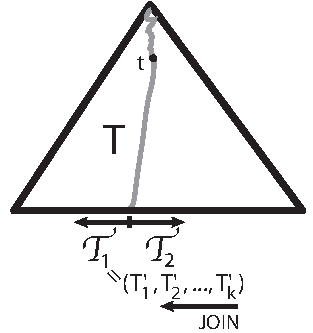
\includegraphics{pics/abtree-split}
\caption{Idea operace SPLIT}
\label{fig:abtree.split}
\end{figure}

Přepis operace SPLIT viz algoritmus \ref{alg:abtree.split}

\begin{algorithm}[!htb]
\caption{SPLIT pro $(a,b)$ stromy}
\label{alg:abtree.split}
\begin{algorithmic}
\ENSURE {Vytvoří 
	$T_1$ reprezentující $\{ s \in S: s < x \}$ a
	$T_2$ reprezentující $\{ s \in S: s > x \}$}
\STATE Nechť $Z_1$ a $Z_2$ jsou prázdné zásobníky
\STATE $t := \text{kořen } T$
\WHILE {$t$ není list}
	\STATE $i := 1$
	\WHILE {$H_t[i] < x \land i < \rho_t$}
		\STATE $i := i + 1$ 
	\ENDWHILE
	\STATE Vytvoř strom $T_1$, jehož kořen %$t_1$
	má syny $S_t[1] \dots S_t[i-1]$
	\STATE Vytvoř strom $T_2$, jehož kořen %$t_2$
	má syny $S_t[i+1] \dots S_t[\rho_t]$
	\IF {$T_1$ není jednoprvkový strom}
		\STATE Push($Z_1, T_1$)
	\ENDIF
        \IF {$T_2$ není jednoprvkový strom}
		\STATE Push($Z_2, T_2$)
	\ENDIF
	\STATE $t := S_t[i]$ 
\ENDWHILE
\IF {$t$ reprezentuje prvek různý od $x$}
	\STATE Udělej z $t$ $(a,b)$ strom a vlož ho
	do příslušného zásobníku.
\ENDIF
\STATE $T_1 := \text{STACKJOIN}(Z_1)$ \COMMENT {viz dále}
\STATE $T_2 := \text{STACKJOIN}(Z_2)$
\end{algorithmic}
\end{algorithm}

\subsubsection{Časová složitost operace SPLIT}

Čas rozřezávání stromu je úměrný jeho hloubce. Celkový čas operace
SPLIT ovšem závisí ještě na složitosti operace STACKJOIN.

% ..........................................................................
\subsection{Algoritmus STACKJOIN($Z$) pro zásobník $(a,b)$ stromů}
\label{abtrees.stackjoin}

Operace STACKJOIN provede JOIN všech (a,b)-stromů uložených na zásobníku.
Výsledkem je jediný (a,b)-strom.

Přepis viz algoritmus \ref{alg:abtree.stackjoin}

\begin{algorithm}[!htb]
\caption{STACKJOIN pro $(a,b)$ stromy}
\label{alg:abtree.stackjoin}
\begin{algorithmic}
\STATE $T := \text{Pop}(Z)$
\WHILE {$Z \ne \emptyset$}
	\STATE $T' := \text{Pop}(Z)$
	\STATE $T := \text{JOIN}(T, T')$
\ENDWHILE
\end{algorithmic}
\end{algorithm}

\subsubsection{Časová složitost operace STACKJOIN}

Nechť $Z$ obsahuje $(a,b)$ stromy $T_1 \dots T_k$, přičemž $T_1$ je
vrchol zásobníku.
Platí
\[
\forall i:\ \text{hloubka }T_i \leq \text{hloubka }T_{i+1}
\]
\begin{align*}
\text{čas STACKJOIN}
 & = \text{hloubka }T_2 - \text{hloubka }T_1 + 1 \\
 & + \text{hloubka }T_3 - \text{hloubka }T_2 + 1 \\
 & + \dots \\
 & + \text{hloubka }T_k - \text{hloubka }T_{k-1} + 1 \\
 & = \text{hloubka }T_k - \text{hloubka }T_1 + \text{počet JOINů} \\
 & = O(\text{hloubka }T) = O(\log |S|)
\end{align*}

Tedy i operace SPLIT vyžaduje čas $O(\log |S|)$.

% ..........................................................................
\subsection{Algoritmus FIND($T, k$) pro $(a,b)$ strom}

Nalezení $k$-tého nejmenšího prvku.

Rozšíříme reprezentaci stromu a každému vnitřnímu vrcholu $v$ přidáme:
\begin{itemize}
\item $K_v[1\ .. \ \rho_v]$: $K_v[i]$ je počet listů
v~podstromu $S_v[i]$ 
\end{itemize}

viz algoritmus \ref{alg:abtree.find}

\begin{algorithm}[!htb]
\caption{FIND pro $(a,b)$ stromy}
\label{alg:abtree.find}
\begin{algorithmic}
\STATE $t := \text{kořen }T$
\WHILE {$t$ není list}
	\STATE $i := 1$
	\WHILE {$K_t[i] < k \land i < \rho_t$}
		\STATE $k := k - K_t[i]$ 
		\STATE $i := i + 1$ 
	\ENDWHILE
	\STATE $t := S_t[i]$ 
\ENDWHILE
\IF {$k > 1$}
	\STATE \textbf{return} nil \COMMENT {$k > |S|$}
\ELSE
	\STATE \textbf{return} $t$
\ENDIF
\end{algorithmic}
\end{algorithm}

Časová složitost je opět logaritmická, přičemž dříve uvedené operace
nejsou zpomaleny tím, že aktualizují pole (seznam) $K$.

% ..........................................................................
\section{A-sort}

Na první pohled se zdá, že použití $(a,b)$ stromů ke třídění není
výhodné. Paměťové nároky budou oproti běžnému třídění v poli asi
pětkrát větší. Aby se tedy třídění $(a,b)$ stromem vyplatilo, muselo
by přinést zvýšení rychlosti. V této části předvedeme, že to skutečně
je možné, jestliže vstupní data jsou již částečně setříděná.

Pro účely A-sortu rozšíříme reprezentaci takto:
\begin{itemize}
\item Listy stromu jsou propojeny do seznamu
\item Je známa cesta z nejmenšího (nejlevějšího) listu do kořene
(uložená např. v zásobníku)
\end{itemize}

Použijeme $(2,3)$-strom. Proč, to si zdůvodníme až po odvození složitosti
A-sortu.

Nechť vstupní posloupnost je $a_1, \dots, a_n$. Postupně odzadu
vkládáme její prvky do stromu modifikovaným INSERTem:

\begin{algorithmic}
\STATE $k := n$
\WHILE {$k > 1$}
	\STATE A-INSERT($a_k$)
	\STATE $k := k - 1$
\ENDWHILE
\end{algorithmic}

Na konci přečteme setříděnou posloupnost pomocí spojového seznamu
listů.

\subsection{A-INSERT}

A-INSERT (viz algoritmus \ref{alg:abtree.a-insert}) pracuje
téměř stejně jako původní INSERT - najde správný list a potom
případně přidá nový prvek. K nalezení správného listu ovšem využívá
cestu z nejmenšího listu. (viz obr. \ref{fig:abtree.a-insert})

\begin{figure} 
\centering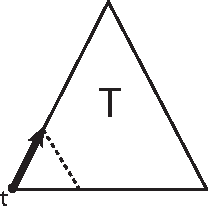
\includegraphics{pics/a-insert}
\caption{Idea algoritmu A-INSERT}
\label{fig:abtree.a-insert}
\end{figure}

Zde uvedená verze A-INSERTu odstraňuje 
duplicitní prvky, operaci lze pochopitelně upravit tak, že nechává 
duplicitní prvky, které zůstávají ve stejném pořadí.

\begin{algorithm}[!htb]
\caption{A-INSERT($x$)}
\label{alg:abtree.a-insert}
\begin{algorithmic}
\STATE \COMMENT {Nalezení}
\STATE $t := \text{nejmenší list stromu } T$
\REPEAT
	\STATE $t := \text{otec } t$
\UNTIL {$t \text{ je kořen} \lor x \leq H_t[1]$}
\STATE \COMMENT {nyní jako v původním INSERTu, pouze jsme jinak
inicializovali $t$}
\WHILE {$t$ není list}
	\STATE $i := 1$
	\WHILE {$H_t[i] < x \land i < \rho_t$}
		\STATE $i := i + 1$
	\ENDWHILE
	\STATE $t := S_t[i]$ 
\ENDWHILE
\STATE \COMMENT {Přidání}
\IF {$t$ nereprezentuje $x$}
	\STATE $o := \text{otec } t$
	\STATE vrcholu $o$ přidej nového syna $t'$ 
	reprezentujícího $x$
	\STATE zařaď $t'$ na správné místo mezi jeho bratry
	a uprav $\rho_o$, $S_o$ a $H_o$
	\STATE $t := o$
	\WHILE {$\rho_t > b$}
		\STATE \COMMENT {Štěpení 
				--- můžeme provést díky podmínce 4}
		\STATE rozděl $t$ na $t_1$ a $t_2$ 
		\STATE \quad k $t_1$ dej prvních 
			$\lfloor (b+1)/2 \rfloor$ synů $t$
		\STATE \quad k $t_2$ dej zbylých 
			$\lceil (b+1)/2 \rceil$ synů $t$
		\STATE $o := \text{otec } t$
		\STATE uprav $\rho_o$, $S_o$ a $H_o$
		\STATE \COMMENT {při štěpení kořene ještě musíme
				vytvořit nový kořen}
	\ENDWHILE
\ENDIF
\end{algorithmic}
\end{algorithm}

\subsection{Složitost A-sortu}

Čas A-sortu
= $\sum$ času vyhledání + $\sum$ času přidání + čas vytvoření výstupní
posloupnosti.
Čas vytvoření výstupní posloupnosti = $O(n)$.

$\sum \text{času přidání} 
= \text{počet přidaných vrcholů} \cdot \text{čas přidání vrcholu}
+ \text{počet štěpení} \cdot \text{čas štěpení}
= O(n) \cdot O(1)
+ \text{počet štěpení} \cdot O(1).$ 
Protože se zde neprovádí operace DELETE, lze každému štěpení přiřadit 
vnitřní vrchol, který byl při tomto štěpení vytvořen (štěpení rozdělí 
vrchol $t$ na dva vrcholy $t_1$ a $t_2$, budeme předpokládat, že 
vrchol $t_1$ je pokračováním vrcholu $t$ a vrchol $t_2$ je vrchol 
vzniklý při štěpení). Tedy počet štěpení je menší než počet vnitřních 
vrcholů (při štěpení kořene vzniká navíc ještě nový kořen),  
tedy $\sum \text{času přidání} = O(n).$

Čas A-sortu tedy závisí hlavně na celkovém čase vyhledání prvků.
Označme
\[
f_i = |\{ j > i:\ a_j < a_i \}|,
\]
tedy počet prvků posloupnosti, které v nesetříděné posloupnosti
následují $a_i$, ale v setříděné patří před $a_i$. Při vyhledání $a_i$
ve stromu vyjadřuje $f_i$ počet listů nalevo od $a_i$. Čas
vyhledání $a_i$ je tedy $O(\log f_i)$ a celkový čas vyhledání je 
$O(\sum \log f_i)$.
\mnote{ošetřit $\log 0$}

Hodnota $F = \sum f_i$, zvaná 
\emph{počet inverzí}, \mnote{nebo transpozic? standardní termín?}%
vyjadřuje uspořádanost vstupní
posloupnosti. Pro správně uspořádanou posloupnost je $F = 0$, pro
obráceně uspořádanou posloupnost je $F = n (n-1) / 2$. To jsou také
mezní hodnoty, jichž může $F$ nabývat.

Z vlastností logaritmu a srovnáním geometrického a aritmetického
průměru dostáváme
\[
\sum \log f_i = \log \prod f_i = n \log \sqrt[n]{\prod f_i}
\leq n \log (F/n).
\]

A-sort tedy vyžaduje čas $O(n \max(1, \log((F+1)/n)))$. V nejhorším
případě to je $O(n \log n)$ a Mehlhorn a Tsakalidis ukázali, že A-sort
je lepší než Quicksort v případě, že $F \leq 0.02 n^{1.57}$.
Naproti tomu Insertsort, jednoduchý algoritmus, který postupně
lineárním prohledáním zatřiďuje prvky pole do jeho již setříděného
počátečního úseku, vyžaduje čas $O(n + F)$, což je v nejhorším případě
$O(n^2)$.

Zbývá ještě zdůvodnit, proč použít $(2,3)$-stromy. Víme, že $(2,3)$-stromy 
mají nejmenší prostorové nároky mezi $(a,b)$-stromy. Na druhé straně však 
$(2,3)$-stromy v obecném přépadě vyžadují zbytečně mnoho vyvažovacích 
operací, a proto jsou výrazně pomalejší než např. $(2,4)$-stromy. Protože 
však A-sort nepoužívá operaci DELETE, ukázali jsme (viz počet operací 
Štěpení), že pro A-sort to není pravda. Zde $(2,3)$-stromy patří mezi 
nejrychleji pracující $(a,b)$-stromy.

% --------------------------------------------------------------------------
\section{Paralelní přístup do $(a,b)$ stromů}

Při operacích INSERT a DELETE jsme nejprve sestupovali stromem dolů až
k listům, potom jsme se vraceli nahoru a štěpili nebo spojovali
vrcholy. To znemožňuje dovolit paralelní přístup do stromu. Procesu,
který je ve fázi vyhledání, by se mohlo stát, že mu jiný proces změní
strom ``pod rukama''. Stávající operace INSERT a DELETE tedy požadují
výlučný přístup ke stromu.
\par
Nyní předvedeme paralelní verzi těchto operací, kde se štěpení nebo
spojování provádí již při sestupu. Potom již není nutné se vracet a je
tedy možné rovnou odemykat části stromu, ke kterým již daný proces
nebude přistupovat. Cenou za tento přístup jsou zbytečná
štěpení/spojení.
\mnote{udělat obrázek ilustrující zbytečná š/s}

Potřebujeme omezit $b$: podmínku $b \geq 2a - 1$ zpřísníme na
\begin{enumerate}
\item[4'.] $a \geq 2$ a $b \geq 2a$ 
\end{enumerate}

% ..........................................................................
\subsection{Paralelní INSERT($x$) do $(a,b)$ stromu}

viz algoritmus \ref{alg:abtree.par.insert}

\begin{algorithm}[!htb]
\caption{paralelní INSERT pro $(a,b)$ stromy}
\label{alg:abtree.par.insert}
\begin{algorithmic}
\STATE $o := \text{lock}(\text{nadkořen})$ \COMMENT {Nadkořen
je implementační pomůcka. Slouží k zamknutí
přístupu k celému stromu a uchovává $\max(S)$}
\STATE $t := \text{kořen}$ 
\STATE \COMMENT {Invariant mezi průchody cyklem:
	$o$ je otec $t$, $o$ je jediný vrchol zamknutý tímto procesem.}
\WHILE {$t$ není list}
	\STATE $i := 1$
	\WHILE {$i < \rho_t \land H_t[i] < x$}
		\STATE $i := i + 1$
	\ENDWHILE
	\STATE $s := S_t[i]$ 
	\STATE \COMMENT {preventivní rozštěpení:}
	\IF {$\rho(t) = b$}
		\STATE rozděl $t$ na $t_1$ a $t_2$: \COMMENT {viz 4'}
		\STATE \quad k $t_1$ dej prvních 
			$\lfloor (b+1)/2 \rfloor$ synů $t$
		\STATE \quad k $t_2$ dej zbylých 
			$\lceil (b+1)/2 \rceil$ synů $t$
		\STATE \quad $t_1$ předchází $t_2$
		\STATE uprav $\rho_o$, $S_o$ a $H_o$
		\STATE \COMMENT {implic.: uprav $\rho_{t_1}$, \dots, $H_{t_2}$}
		\STATE \COMMENT {při štěpení kořene ještě musíme
				vytvořit nový kořen}
		\STATE $n := t_j$, kde $s$ je syn $t_j$
	\ELSE
		\STATE $n := t$
	\ENDIF
	\STATE lock($n$) 
	\STATE unlock($o$) 
	\STATE $o := n$
	\STATE $t := s$
\ENDWHILE
\IF {$t$ nereprezentuje $x$}
	\STATE vrcholu $o$ přidej nového syna $t'$ 
	reprezentujícího $x$
	\STATE zařaď $t'$ na správné místo mezi jeho bratry
	a uprav $\rho_o$, $S_o$ a $H_o$
\ENDIF
\STATE unlock($o$)
\end{algorithmic}
\end{algorithm}

% ..........................................................................
\subsection{Paralelní DELETE($x$) z $(a,b)$ stromu}

viz algoritmus \ref{alg:abtree.par.delete}

\begin{algorithm}[!htb]
\caption{paralelní DELETE pro $(a,b)$ stromy}
\label{alg:abtree.par.delete}
\begin{algorithmic}
\STATE $o := \text{lock}(\text{nadkořen})$ \COMMENT {Nadkořen
je implementační pomůcka. Slouží k zamknutí
přístupu k celému stromu a uchovává $\max(S)$}
\STATE $t := \text{kořen}$ 
\STATE $h := \textbf{nil}$ \COMMENT 
	{Jakmile $h \neq \textbf{nil}$, 
	$x \in H_h$ a $h$ bude zamčený do konce procesu.}
\STATE \COMMENT {Invariant mezi průchody cyklem:
	$o$ je otec $t$, $o$ je kromě $h$ jediný vrchol
	zamknutý tímto procesem.}
\WHILE {$t$ není list}
	\STATE $i := 1$
	\WHILE {$i < \rho_t \land H_t[i] < x$}
		\STATE $i := i + 1$
	\ENDWHILE
	\IF {$H_t[i] = x$}
		\STATE $h := t$
	\ENDIF
	\STATE $s := S_t[i]$ 
	\STATE \COMMENT {preventivní spojení/přesun:}
	\IF {$\rho(t) = a$}
		\STATE $v := \text{bezprostřední bratr } t$ %bratr[fi]=_v_eli
		\IF[smíme spojit] {$\rho_v = a$}
			\STATE \COMMENT {Spojení}
			\STATE sluč $v$ a $t$ do $t$ \COMMENT {viz 4'}
			\STATE uprav $\rho_o$, $S_o$ a $H_o$
			\STATE $t := o$
		\ELSE[$\rho_v > a$, spojení by mělo více než $b$ synů]
			\STATE \COMMENT {Přesun}
			\STATE přesuň krajního syna $v$ do $t$
			\STATE uprav $H_o$, $H_v$ a $H_t$
		\ENDIF
	\ENDIF
	\STATE lock($t$) 
	\IF {$o \neq h$}
		\STATE unlock($o$)
	\ENDIF
	\STATE $o := t$
	\STATE $t := s$
\ENDWHILE
\IF {$t$ reprezentuje $x$}
	\STATE odstraň $t$
	\STATE uprav $H_o$, $H_h$
	\STATE uprav $S_o$ a $\rho_o$
	\STATE unlock($h$)
\ENDIF
\STATE unlock($o$)
\end{algorithmic}
\end{algorithm}


% --------------------------------------------------------------------------
\section{Složitost posloupnosti operací na $(a,b)$ stromu}

A-sort funguje jednak proto, že v předtříděné posloupnosti rychle
najde místo, kam se má vkládat, jednak proto, že se při samých
INSERTech ({\it a díky správným $a$, $b$?}) provádí málo
vyvažovacích kroků. V této sekci se podíváme na počet vyvažovacích
kroků pro posloupnost operací INSERT a DELETE.

Nechť $b \geq 2a$.
\begin{theorem}
Mějme posloupnost $n$ operací INSERT a DELETE aplikovanou na prázdný
$(a,b)$ strom. Označme $P$ počet přesunů při provádění posloupnosti,
$SP$ počet spojení a $ST$ počet štěpení. Dále označme $P_h$, $SP_h$ a
$ST_h$ počet přesunů. spojení a štěpení, které nastanou ve výšce $h$
(listy mají výšku 0).

Nechť
\begin{equation}
\begin{split}
% this is ``occult alignment'' :)
c = \min
 &\left(
   \phantom{b - \vphantom{x}}
        \min \left( 2a-1, \left\lceil \frac{b+1}{2}\right\rceil  \right) - a, 
  \right.\\
 &\left.
		\phantom{\left(
		\vphantom{\left. \frac xy\right.}
		\right.}
    b - \max \left( 2a-1, \left\lfloor\frac{b+1}{2}\right\rfloor \right)
   \phantom{\vphantom{x} - a}
  \right)
\end{split}
\end{equation}

Pak platí
%\renewcommand{\labelenumi}{\alph{enumi}}
\begin{eqnarray}
P &\leq& n \\
\label{ab-v-stsp}
(2c-1)ST + cSP &\leq& n + c + \frac c{a+c-1} (n-2) \\
\label{ab-v-sthsph}
P_h + SP_h + ST_h &\leq& \frac{2 n^{c+2}}{(c+1)^h} 
\end{eqnarray}
\end{theorem}

Platí $c \geq 1$ (při $b = 2a$ dokonce $c = 1$). Z toho
\begin{equation}
ST + SP \leq \frac nc + 1 + \frac{n-2}a,
\end{equation}
tedy lineárně vzhledem k $n$.

Pro paralelní verze INSERT a DELETE platí obdobná věta, když 
$b \geq 2a + 2$.

Pro důkaz použijeme \emph{bankovní paradigma}: datovou strukturu
ohodnotíme podle toho, jak je ``uklizená''. Operace, které datovou
strukturu ``uklidí'', zvětší její ``zůstatek na účtě''. Ty, které ji
``naruší'', zůstatek zmenší. Potom najdeme vztah mezi zůstatkem a
spotřebovaným časem.
{\it Tohle pokulhává. Myslel jsem si, že zůstatek je něco jako čas v
konzervě, který si pomalé operace berou od rychlých \dots, ale  v
tomhle případě to asi funguje jinak.}
\mnote{vyjasnit}
\mnote{použiju $z$ jako zůstatek místo $b$ jako balance, protože
souvislost s vyvažováním stromu je zde spíš matoucí}

$(a,b)$ stromy jsou uklizené, když mají vrcholy počet synů někde
uprostřed mezi $a$ a $b$. Tehdy nenastane v brzké době vyvažovací
operace. V tomto smyslu definujme:
\begin{align}
z(v) &=
	\min ( \rho_v - a, b - \rho_v, c ) 
	&&\text{$v$ je vnitřní vrchol různý od kořene}\\
z(\text{kořen}) &=
        \min ( \rho_v - 2, b - \rho_v, c ) 
\end{align}

Pro strom $T$ definujme 
\[
z(T) = \sum_{v \in T} z(v)
\]
\[
z_h(T) = \sum_{\substack{v \in T\\v \text{ má výšku } h}} z(v)
\]
Platí
\[
z(T) = \sum_h z_h(t)
\]

Podobně jako u červenočerných stromů definujme parciální $(a,b)$-strom:
\begin{defn}
$(T,v)$ je \emph{parciální $(a,b)$-strom,} když $v$ je vnitřní vrchol $T$
různý od kořene a
kromě $v$ jsou splněny podmínky pro $(a,b)$-strom a
$a-1 \leq \rho_v \leq b+1$.
\end{defn}

Z definice zůstatku vyplývají tyto vlastnosti:
\begin{align}
\label{ab-1}
  \rho_v = a-1 \text{ nebo }b+1 &\implies z(v) = -1\\
\label{ab-0}
  \rho_v = a \text{ nebo } b    &\implies z(v) = 0\\
\label{ab-spojeni}
  \rho_v = 2a-1                 &\implies z(v) = c\\
\label{ab-stepeni}
  \rho_u = \left\lfloor\frac{b+1}{2}\right\rfloor \land
  \rho_v = \left\lceil \frac{b+1}{2}\right\rceil
                                &\implies z(u)+z(v) \geq 2c - 1\\
\label{ab-presun}
  |\rho_u - \rho_v| \leq 1      &\implies z(u) \geq z(v) - 1
\end{align}

\subsection{Přidání/ubrání listu}

Mějme $(a,b)$-strom $T$ a přidáme nebo ubereme list, jehož otec je $v$.
Pak vznikne parciální $(a,b)$-strom $(T',v)$ a platí:
\begin{align}
  z_1(T')        & \geq z_1(T) - 1\\
  z_h(T')        & = z_h(T) \quad h>1\\
  z(T')          & \geq z(T) - 1
\end{align}

\subsection{Štěpení}

Mějme parciální $(a,b)$-strom $(T,v)$, kde $v$ je ve výšce $h$.
Nechť $T'$ vznikl \emph{štěpením $v$}. 
Pak $(T',\text{otec }v$ je parciální $(a,b)$-strom a platí:
\begin{align}
  z_h(T')       & \geq 2c + z_h(T)
	\qquad\text{z \ref{ab-1} a \ref{ab-stepeni}}\\
  z_{h+1}(T')   & \geq z_{h+1}(T) - 1\\
  z_i(T')       & = z_i(T) \quad i \neq h, h+1\\
  z(T')         & \geq z(T) + 2c - 1
\end{align}

\subsection{Spojení}

Mějme parciální $(a,b)$-strom $(T,v)$, kde $\rho_v = a-1$ a 
$v$ je ve výšce $h$, $y$ je bezprostřední bratr $v$.
Nechť $\rho_y = a$ a $T'$ vznikl \emph{spojením $v$ a $y$}. 
Pak $(T',\text{otec }v$ je parciální $(a,b)$-strom a platí:
\begin{align}
  z_h(T')       & \geq c + 1 + z_h(T)
	\qquad\text{z \ref{ab-1}, \ref{ab-0} a \ref{ab-spojeni}}\\
  z_{h+1}(T')   & \geq z_{h+1}(T) - 1\\
  z_i(T')       & = z_i(T) \quad i \neq h, h+1\\
  z(T')         & \geq z(T) + c
\end{align}

\subsection{Přesun}

Mějme parciální $(a,b)$-strom $(T,v)$, kde $\rho_v = a-1$ a 
$v$ je ve výšce $h$, $y$ je bezprostřední bratr $v$.
Nechť $\rho_y > a$ a $T'$ vznikl \emph{přesunem syna od $y$ k $v$}. 
Pak $T'$ je $(a,b)$-strom a platí:
\begin{align}
  z_h(T')       & \geq z_h(T)
	\qquad\text{z \ref{ab-1}, \ref{ab-0} a \ref{ab-presun}}\\
  z_i(T')       & = z_i(T) \quad i \neq h\\
  z(T')         & \geq z(T)
\end{align}

Nechť po skončení posloupnosti operací máme $(a,b)$-strom $T_k$.
Sečteme předchozí výsledky:
\begin{equation}
\label{eq:ab-secti}
  z(T_k) \geq (2c - 1)ST + c SP - n  
\end{equation}

\begin{align}
  z_1(T_k)      & \geq 2c ST_1 + (c+1) SP_1 - n\\
  z_h(T_k)      & \geq 2c ST_h + (c+1) SP_h - ST_{h-1} - SP_{h-1} \quad h>1
\end{align}
Vadí nám, že jsou ve výrazu i spojení a štěpení z jiné hladiny.

$c \geq 1 \implies 2c \geq c+1$.
\[
  z_h(T_k) \geq (c+1) (ST_h + SP_h) - ST_{h-1} - SP_{h-1}
\]
\begin{align}
  ST_h + SP_h 
&  \leq \frac{z_h(T_k)}{c+1} + \frac{ST_{h-1} + SP_{h-1}}{c+1}
  \leq \frac{z_h(T_k)}{c+1} + 
         \frac{z_{h-1}(T_k)}{(c+1)^2} + 
         \frac{ST_{h-2} + SP_{h-2}}{(c+1)^2}\\
&  \leq \left( \sum_{i=0}^{h-1} \frac{z_{h-i}(T_k)}{(c+1)^{i+1}} \right) + 
         \frac{ST_0 + SP_0}{(c+1)^h}
                \qquad\text{$j=h-i$, rozšíříme $(c+1)^{h-i}$}\\
\label{ab-sthsph}
&  = \left( \sum_{j=1}^h \frac{z_j(T_k)(c+1)^j}{(c+1)^{h+1}} \right) + 
         \frac{n}{(c+1)^h}
\end{align}

Nechť $T$ je $(a,b)$-strom s $m$ listy. Chceme shora odhadnout $z(T)$.
\begin{equation}
  m_j = \text{počet vnitřních vrcholů různých od kořene}
  \begin{cases}
    \text{s právě $a+j$ syny}   & \text{když}\ j \in\intrange{0}{c-1}\\
    \text{s alespoň $a+j$ syny} & \text{když}\ j = c
  \end{cases}
\end{equation}

Když $v$ je vnitřní vrchol různý od kořene s právě $a+j$ syny,
$j \in\intrange{0}{c-1}$,
pak $z(v) \leq j$.

Když $v$ je vnitřní vrchol různý od kořene s alespoň $a+c$ syny,
pak $z(v) \leq c$.

Tedy
\begin{equation}
  \label{eq:ab-mj}
  z(T) \leq c + \sum_{j=0}^c j m_j = *
\end{equation}

Spočítáme hrany v $T$: nalevo jsou hrany vycházející z kořene a
vnitřních vrcholů, napravo jsou hrany přicházející do vnitřních
vrcholů a listů.
\begin{equation}
2 + \sum_{j=0}^c (a+j) m_j \leq
\text{počet hran}
= \left( \sum_{j=0}^c m_j \right) + m
\end{equation}
Tedy $m-2 \geq \sum_{j=0}^c (a+j-1) m_j$.

\begin{equation}
  *
  =    c + \sum_{j=0}^c \frac{j}{a+j-1}(a+j-1) m_j 
  \leq c + \sum_{j=0}^c \frac{c}{a+c-1}(a+j-1) m_j 
  \leq c + \frac{c}{a+c-1} (m-2)
\end{equation}

Spojením tohoto výsledku s \ref{eq:ab-secti} dostaneme \ref{ab-v-stsp}.

K důkazu \ref{ab-v-sthsph} využijeme \ref{ab-sthsph}.
\begin{equation}
  m_{h,j} = \text{počet vnitřních vrcholů ve výšce $h$}
  \begin{cases}
    \text{s právě $a+j$ syny}   & \text{když}\ j \in\intrange{0}{c-1}\\
    \text{s alespoň $a+j$ syny} & \text{když}\ j = c
  \end{cases}
\end{equation}

\begin{equation}
  z_h(T) \leq \sum_{j=0}^c j m_{h,j}
\end{equation}
\begin{equation}
  \sum_{j=0}^c m_{h,j}
   = \text{počet vrcholů ve výšce $h$} 
  \geq \sum_{j=0}^c (a+j) m_{h+1,j}
\end{equation}
\begin{equation}
\label{ab-x}
  \sum_{j=0}^c j m_{h,j}
  \leq \sum_{j=0}^c m_{i-1,j} - a \sum_{j=0}^c m_{i,j} 
\end{equation}
\begin{align}
   \sum_{i=1}^h z_i(T_k)(c+1)^i
 & \leq \sum_{i=1}^h (c+1)^i \left( \sum_{j=0}^c j m_{i,j} \right) \\
\intertext{označme $s_i = \sum_{j=0}^c m_{i,j}$}
 & \stackrel{\text{\ref{ab-x}}}{\leq} 
        \sum_{i=1}^h (c+1)^i \left( s_{i-1} - a s_i \right) \\
 & = (c+1)s_0 - (c+1)^h a s_h + 
        \sum_{i=2}^h (c+1)^i \left( s_{i-1} - \frac{a}{c+1} s_{i-1} \right) \\
 & \leq (c+1) m \qquad\text{protože $\frac{a}{c+1} \geq 1$ a $s_0 = m$}
\end{align}

\[
ST_h + SP+h \leq \frac{m}{(c+1)^h} + \frac{n}{(c+1)^h} \leq \frac{2n}{(c+1)^h}
\]
\[
P_h \leq SP_{h-1} - SP_h \leq SP_{h-1} + ST_{h-1} \leq \frac{2n}{(c+1)^{h-1}}
\]
Tím dostáváme \ref{ab-v-sthsph}:
\[
ST_h + SP_h + P_h \leq \frac{2 n (c+2)}{(c+1)^h}
\]


% --------------------------------------------------------------------------
\section{Propojené $(a,b)$ stromy s prstem}

Variantou $(a,b)$ stromů jsou $(a,b)$ stromy, které mají propojené
jednotlivé hladiny a dále obsahují ukazatel na jeden z listů.
Těmto stromům se také někdy říká jenom stromy s prstem (předpokládá se, že
jsou propojené) nebo hladinově propojené. V anglické literatuře se
vyskytují pod pojmem \emph{finger trees}.
\par
Struktura vnitřního vrcholu $v$ obsahuje následující položky: 
\begin{itemize}
\item $\rho(v) =$ počet synů $v$ 
\item $Syn[1..\rho(v)]$ je pole ukazatelů na syny vrcholu $v$
\item $Hod[1..\rho(v)]$ je pole hodnot, platí 
\item $Hod(i-1) <$ prvky reprezentované v podstromu $i$-tého syna $\leq Hod(i)$ 
\item $otec(v)$ = ukazatel na otce vrcholu $v$
\end{itemize}

\begin{tabular}{l}
Předchůdce$(v)$ \\
Následník$(v)$
\end{tabular}
$\Bigl\}$
\begin{tabular}{l}
ukazatele na bezprostř. předchůdce (následníka) v na hladině vrcholu $v$ \\
(v lexikogr. uspořádání)
\end{tabular}
\par

$h$ - hodnota, která leží mezi největším prvkem podstromu v a nejmenším
prvek podstromu následníka.

Příklad (a,b)-stromu s prstem je vidět na obr. \ref{fig.abtree.finger}

\begin{figure}[!htb]
\centering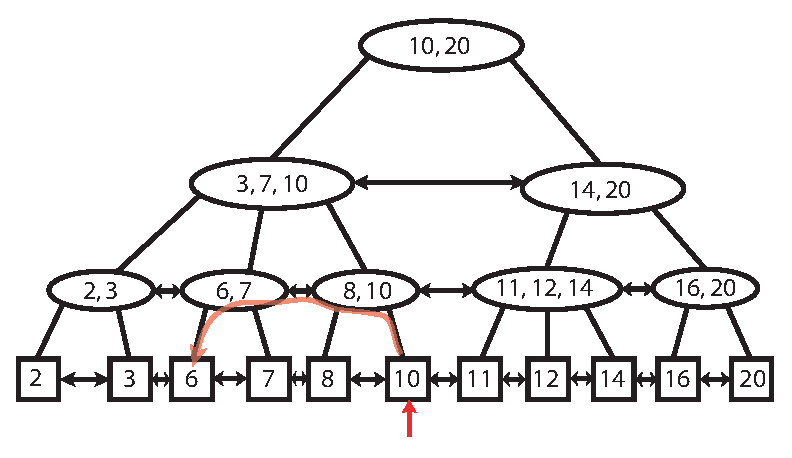
\includegraphics{pics/abtree-finger}
\caption{(a,b)-strom s prstem při provedení operace MEMBER(6)} 
\label{fig.abtree.finger}
\end{figure} 

\subsection{Algoritmus MEMBER}

Viz algoritmus \ref{alg:abtreesfing.member}

\mnote{XXX alg. MEMBER je velmi podivny, prepracovat}

\begin{algorithm}[!htb]
\caption{MEMBER (a,b) stromy s prstem}
\label{alg:abtreesfing.member}
\begin{algorithmic}
\STATE MEMBER(x)
\STATE 1) Nechť $y$ je hodnota, na kterou ukazuje Prst.
  \IF {$x < y$} 
    \STATE pokračuju 2)
  \ELSE
    \STATE 3)
  \ENDIF
\STATE 2) $v \leftarrow otec(y)$
  \STATE dokud $x < h$(Předchůdce(Předchůdce($v$))
   \STATE jdu na otce(Předchůdce($v$))
  \STATE v opačném případě
    \STATE když $x \leq$ h(Předchůdce($v$)) pak
    \STATE $v$ $\leftarrow$ Předchůdce($v$)
    \STATE a pokračuji normálním vyhledáváním
\STATE 3) symetrické ke 2)
\end{algorithmic}
\end{algorithm}

\subsection{Algoritmus FINGER}

FINGER($x$) \\
nastaví hodnotu na list, který reprezentuje prvek nejbližší k x.

Použití: \\
když lze operace přirozeným způsobem rozdělit do segmentů a operace v ?
segmentu mají operace blízko sebe
\par

\begin{itemize}
\item vyhledání $x$ vyžaduje čas $O(1 + \log(l))$
\item nastavím prst na nějakou vhodnou hodnotu
\end{itemize}

\begin{theorem}
Nechť $T$ je propojovaný (a,b) strom s prstem a nechť $P$ je posloupnost
příkazů MEMBER, INSERT, DELETE, FINGER, kterou provedeme na $T$.
Pak $P$ vyžaduje čas $O(log(n) + \text{čas na vyhledání})$
kde $n$ je velikost množiny reprezentované stromem $T$. ($b \geq 2a$)
\end{theorem}

\subsection{Amortizovaná složitost}

Vezmeme posloupnost $n$ operací, spočítáme maximální čas, který vyžadují a
ten vydělíme $n$. 
Limita takto získaných čísel pro $n \rightarrow \infty$ je amortizovaná
složitost.

\subsubsection{Bankovní paradigma}

Použijeme následující značení pro přechodu mezi stavy (situacemi):
$D \stackrel{o}{\rightarrow} D'$

\begin{itemize}
\item $D$ - vstupní situace 
\item $o$ - operace 
\item $D'$ - výstupní operace 
\end{itemize}

Amortizovaná složitost operace $o$ je Čas$(O) + bal(D') - bal(D)$,
kde $bal()$ je ohodnocení konfigurace.

$D_0 \stackrel{O_1}{\rightarrow} D_1 \stackrel{O_2}{\rightarrow} D_2 \rightarrow \ldots \rightarrow D_n$

$$\sum_{i=1}^{n} \text{čas}(O_i) + bal(D_n) - bal(D_0) = \sum a(O_i) \leq
\sum i(O_i)$$

Obvykle platí, že $bal \geq 0$ nebo $bal \leq 0$. \\
Když $bal \geq 0$, pak: \\
  $$\sum \text{čas}(O_i) \leq \sum a(O_i) + bal(D_0) \leq \sum i(O_i) + bal(D_0)$$
Když $bal \leq 0$, pak \\
  $$\sum \text{čas}(O_i) \leq \sum a(O_i) - bal(D_n) \leq \sum i(O_i) - bal(D_0)$$

Začínáme na prázdném (a,b) stromě $\rightarrow bal = 0$.

XXX nechybi tady neco ?


